\documentclass[twocolumn]{article}

\title{Orientation and design of LPC1769 CAN Bootloader}
\author{Chiel de Roest\\4036832 \and Harmjan Treep\\4011724}
\date{}

\usepackage[english]{babel}
\usepackage[pdfborder={0 0 0},plainpages=false]{hyperref}
\usepackage{fullpage}
\usepackage{graphicx}
\usepackage{tikz}
\usepackage{pgf-umlsd}
\usepackage{amsmath}
\usetikzlibrary{arrows,shadows}

% Hack to create memory diagrams inspired by http://www.martin-demling.de/2011/06/memory-maps-in-latex-using-the-bytefield-package/
\usepackage{bytefield}
\newcommand{\memsection}[4]{
	%\bytefieldsetup{bitheight=#3\baselineskip}    % define the height of the memsection
	\setlength{\byteheight}{#3\baselineskip}
	\bitbox[]{10}{
		\texttt{#1} \\[#3\baselineskip] \vspace{-2.2\baselineskip} \texttt{#2} % print start address
	} 
	\bitbox{14}{#4} \\ % print box with caption
}

\newcommand{\protospace}{\textit{proto}SPACE }

\begin{document}

\maketitle

\begin{abstract}
	Our main assignment is to implement tools to develop with on the \protospace floor.
	The first subproject was to build a CAN Bootloader for the LPC1769 and in this document will we discuss how we approached this problem and what design considerations we took into account.
\end{abstract}

\section*{Orientation}
	To orient ourselves on the assignment of implementing a CAN bootloader we did an example project.
	We implemented a CAN driver for the LPC1769 in the CMSIS library from NXP with the LPCXpresso shield as hardware platform,
	this is exactly the hardware platform that is planned to be installed in the floor of the \protospace room.
	After some struggling we managed to implement a new project which could send and receive messages on the CAN bus.
	
	\subsection*{Platform}
		The hardware platform for our project is the LPCXpresso LPC1769.
		This board is plugged into a custom developed board called the LPCXpresso shield.
		We worked on the first version of the hardware board,
		in the new version only minor bugs are fixed and the board is physically smaller overall.
		
		We worked with the assembly as seen in \autoref{fig:shield}.
		An assembly very much alike this one will be implemented in the \protospace floor.
		\begin{figure}[htbp]
			\centering
			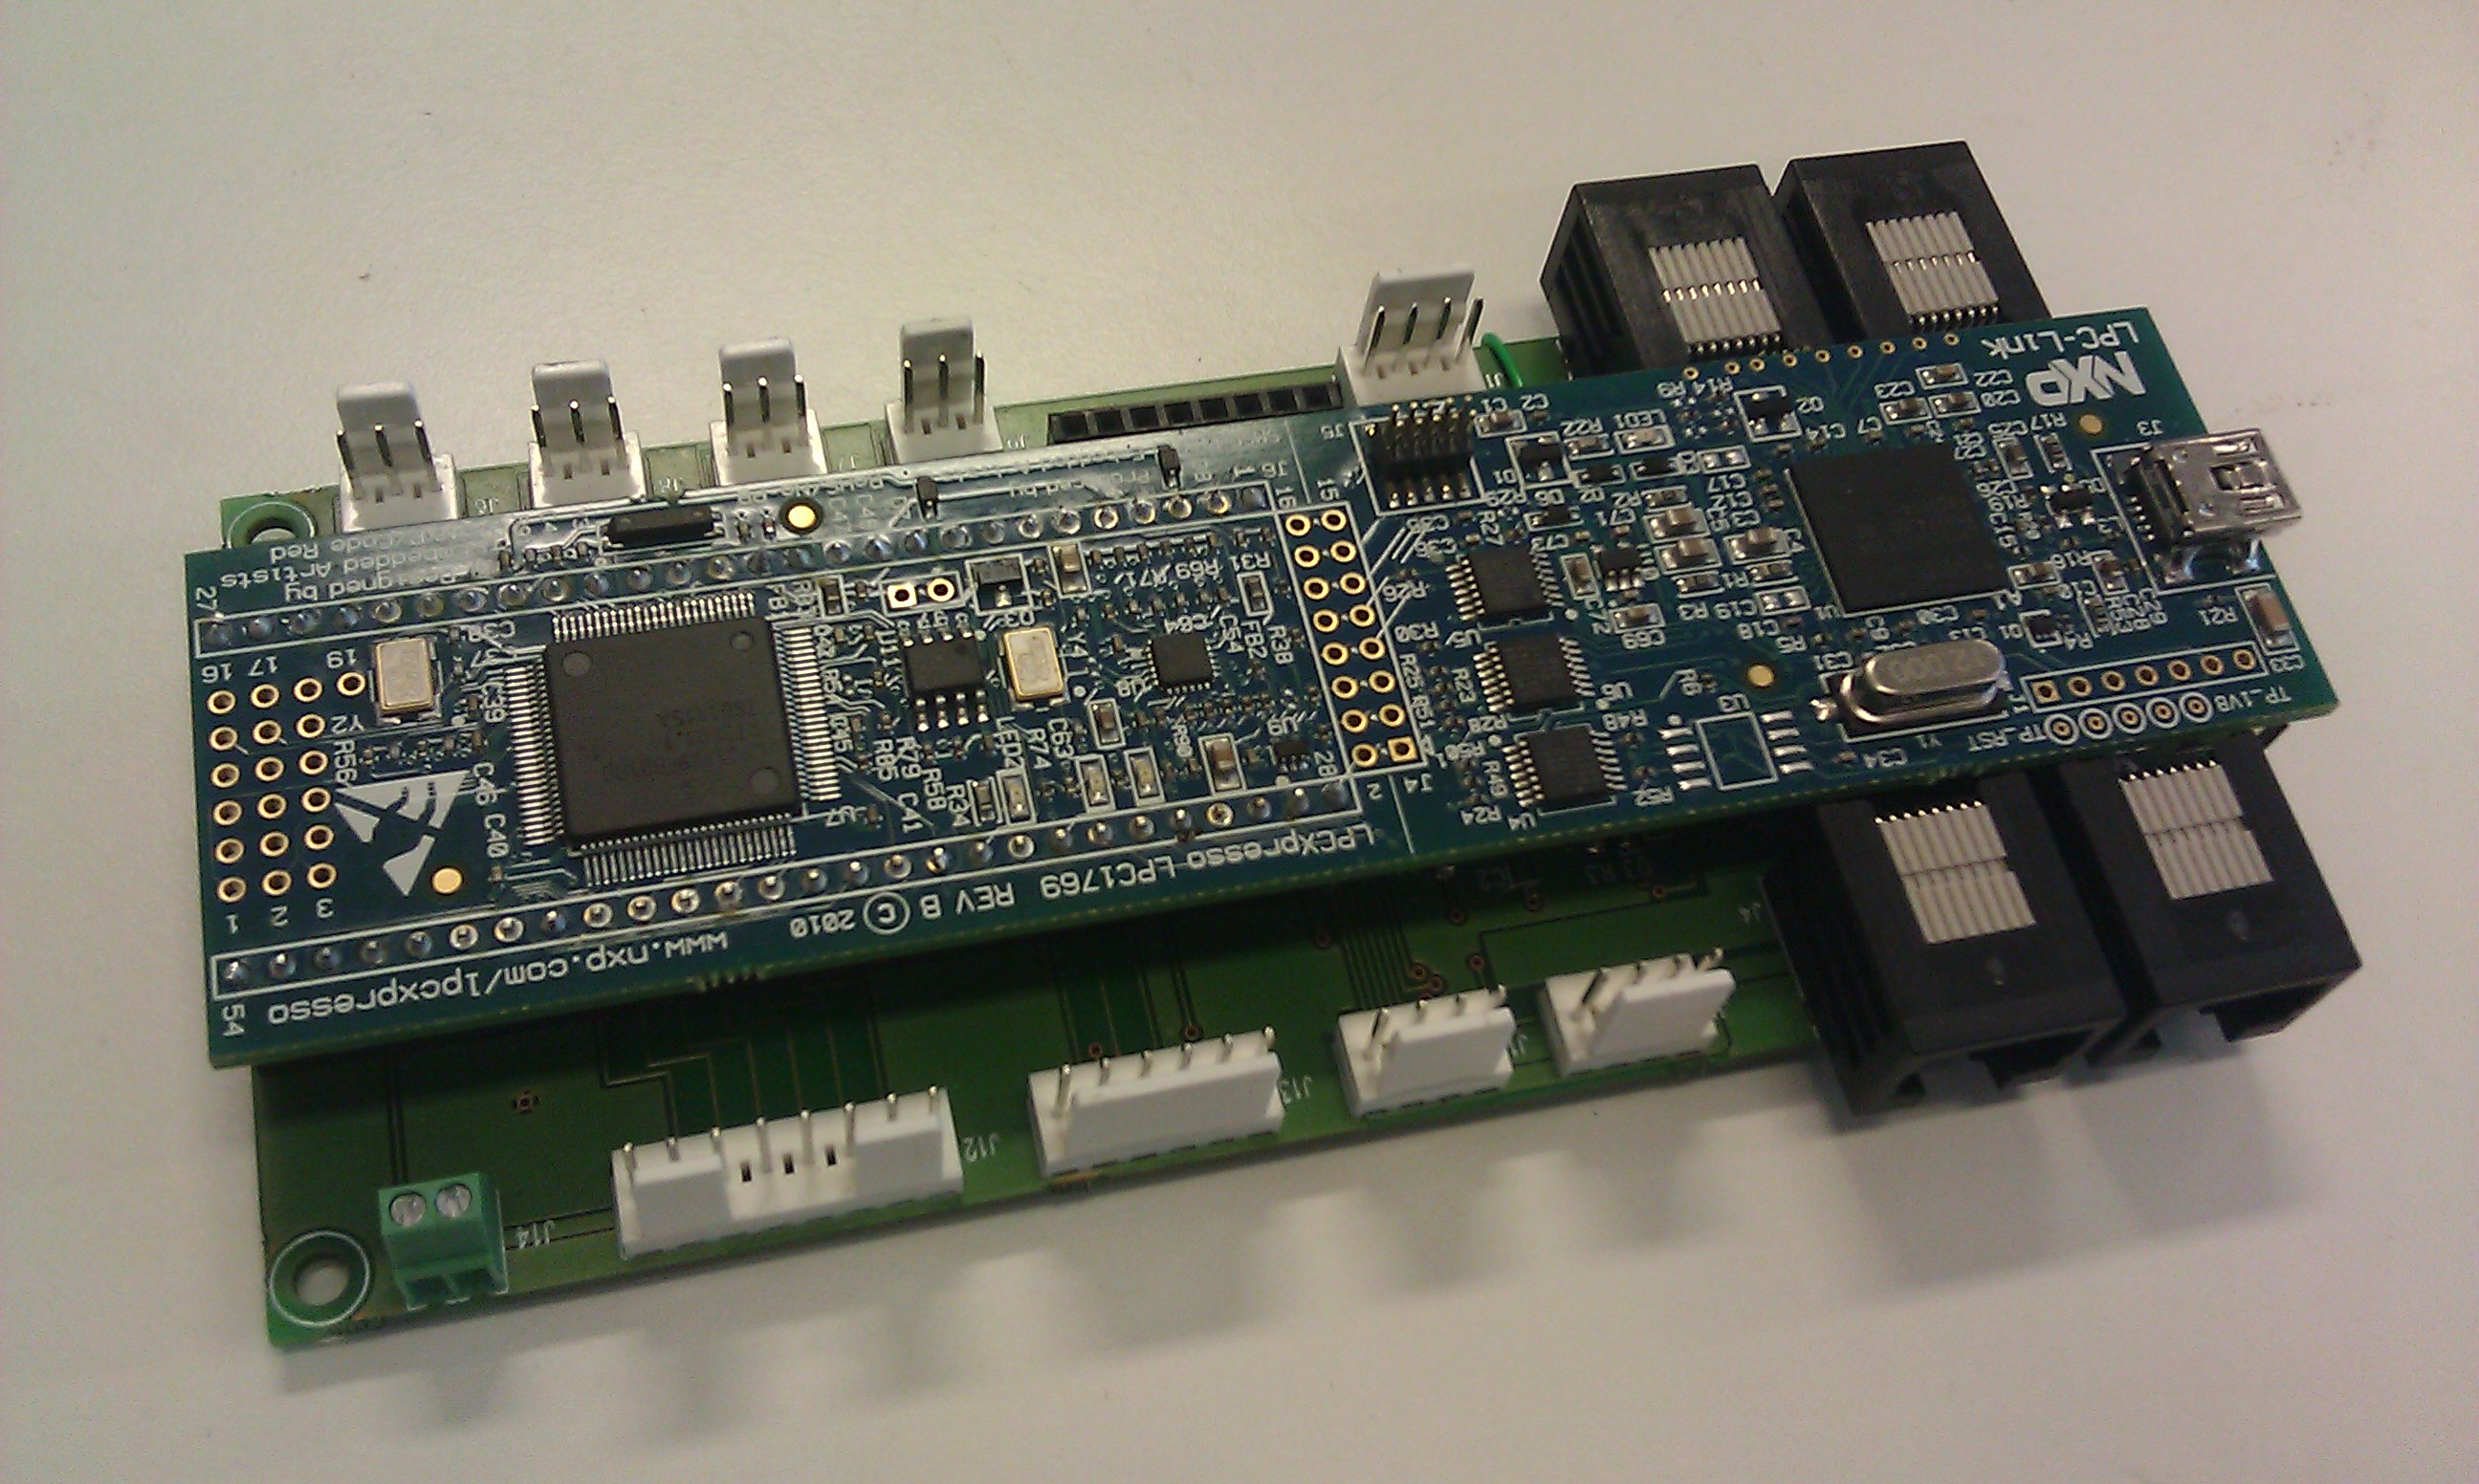
\includegraphics[width=\columnwidth]{LPCXpressoShieldAssembly}
			\caption{The LPCXpresso LPC1769 and the LPCXpresso shield V1 assembly}
			\label{fig:shield}
		\end{figure}
		
		The boards are connected with their neighbours via UART and all boards are also connected to each other via a single CAN bus,
		as seen in \autoref{fig:network}.
		\begin{figure}[htbp]
			\centering
			\tikzstyle{square}=[rectangle,thick,minimum size=0.5cm,draw=black]
			\begin{tikzpicture}[auto, outer sep=3pt, node distance=2cm,>=latex']
				\node [square] (1) {Node 1};
				\node [square] (2) [right of=1] {Node 2};
				\node [square] (3) [right of=2]{Node 3};
				\node [square] (4) [below of=1]{Node 4};
				\node [square] (5) [right of=4]{Node 5};
				\node [square] (6) [right of=5]{Node 6};
				\node [square] (7) [below of=4]{Node 7};
				\node [square] (8) [right of=7]{Node 8};
				\node [square] (9) [right of=8]{Node 9};
			
				\draw [<->,thick] (1) --  node {} (2) ;
				\draw [<->,thick] (2) --  node {} (3) ;
				\draw [<->,thick] (1) --  node {} (4) ;
				\draw [<->,thick] (2) --  node {} (5) ;
				\draw [<->,thick] (3) --  node {} (6) ;
				\draw [<->,thick] (4) --  node {} (5) ;
				\draw [<->,thick] (5) --  node {} (6) ;
				\draw [<->,thick] (4) --  node {} (7) ;
				\draw [<->,thick] (5) --  node {} (8) ;
				\draw [<->,thick] (6) --  node {} (9) ;
				\draw [<->,thick] (7) --  node {} (8) ;
				\draw [<->,thick] (8) --  node {} (9) ;
			
				\path[red,thick] (7) edge [bend left] node {} (4)
				      (4) edge [bend left] node {} (1)
				      (1) edge [bend left] node {} (2)
				      (2) edge [bend right] node {} (5)
				      (5) edge [bend right] node {} (8)
				      (8) edge [bend right] node {} (9)
				      (9) edge [bend left] node {} (6)
				      (6) edge [bend left] node {} (3);
			\end{tikzpicture}
			\caption{A sensor node network with a CAN bus}
			\label{fig:network}
		\end{figure}
		
		CAN is a communication protocol implementing the lowest two layers in the OSI network layer model.
		CAN works by setting messages with an 11 bit ID and up to 8 bytes of data on the bus.
		Every node on the bus receives every message.
		
		The department wants to be able to load applications onto the nodes in the \protospace floor without having to lift any tiles.
		That is why they want a CAN bootloader.
	
	\subsection*{Tools}
		The LPCXpresso platform comes with an IDE.
		This IDE is especially good for debugging code for the LPCXpresso:
		you can set breakpoints and step through the code while visually inspecting all the registers.
		The IDE will be very helpful while developing the CAN bootloader.
		
		The LPCXpresso IDE is free to use for programs that are smaller than 128kB.
		The department however wants to develop for the nodes in a high level language like eLua or proto,
		which means that they want to flash a large image with the virtual machine onto the nodes.
		To circumvent this restriction they utilize the built-in UART bootloader of the LPC1769.
		To work with the UART bootloader they use cables to communicate between the computer and processor over UART.
		These cables can also be used to send debug information between the hostcomputer and the processor.
		We can keep this in mind while developing for the LPC1769.
		
		The department has 2 Saleae Logic's which are logic analyzers.
		With those logic analyzers we can monitor signals in the hardware which is very useful while debugging.
	
	\subsection*{Facilties}
		The faculty has an electronics room with most common equipment like soldering irons, breadboards and jumper wires.
		We can use these as we like for making test setups for the node.

\section*{Design}
	After the orientation project we focussed on the main problem: the CAN bootloader for the LPC1769.
	We tried to do a complete as possible design of the software before starting implementation of the bootloader.
	
	\subsection*{Overview LPC1769}
		The memory of the LPC1769 looks like \autoref{fig:flash}.
		Our program must reside in the Flash memory along with the user program.
		\begin{figure}[htbp]
			\centering
			\begin{bytefield}{24}
				\memsection{0x1000 7FFF}{0x1000 0000}{5}{Local Static RAM}
				\memsection{0x0FFF FFFF}{0x0008 0000}{5}{\textit{reserved}}
				\memsection{0x0007 FFFF}{0x0000 0401}{5}{Flash Memory}
				\memsection{0x0000 0400}{0x0000 0008}{3.2}{Interrupt vector table}
				\memsection{0x0000 0007}{0x0000 0004}{2.2}{Stack pointer}
				\memsection{0x0000 0003}{0x0000 0000}{2.2}{Start pointer}
			\end{bytefield}
			\caption{Relevant parts of the LPC1769 memory}
			\label{fig:flash}
		\end{figure}
		
		The LPC1769 has a lot of built-in peripherals,
		which are hardware functionalities.
		One can interact with these peripherals via registers.
		The CAN peripheral consists of 2 registers, which are needed to be used to perform all functionality.
		Implementing all functionality can be done with interrupts or by polling the registers.
		In the case of polling the registers, it is called a blocking implementation since no other function can be performed by the processor while waiting for something.
	
	\subsection*{Functions and requirements}
		After analysis of what the bootloader was supposed to do we defined the following main function.
		\begin{quote}
			A bootloader can update the user program in flash memory.
		\end{quote}
		We use the bootloader as the program that can flash the node and the user program as the program that is flashed by the bootloader.
		After functional analysis of the problem we identified requirements to within implement the bootloader.
		\begin{itemize}
			\item The bootloader must work on the LPCXpresso LPC1769.
			\item The bootloader must be able to flash the node while the programmer can only communicate with the node over CAN.
			\item The bootloader must be able to program one specific node in the network.
			\item The bootloader must be able to detect which nodes in the network are in bootloading mode.
			\item The node must be able to go into bootloading mode from all states of the user program.
			\item The bootloader should be able to detect all nodes in the network with the bootloader software.
			\item The bootloader should be able to detect write errors and be able to communicate them to the programmer.
			\item The bootloader should use as little ROM memory as possible.
			\item The bootloader should be as transparent as possible to the programmer that uses the bootloader.
				With this requirement we mean that the programmer that is using this bootloader shouldn't have to think about it,
				he should not notice that there is a bootloader in the ROM where his program also is.
			\item Flashing all 200 nodes in the network should be able to be done in less than 5 minutes.
		\end{itemize}
		
		We will discuss how we are planning on implementing different aspects of the bootloader and why we want to do it that way.
	
	\subsection*{Location of the bootloader}
		The bootloader has to be in ROM with the user program, there is no other option.
		For the place of the bootloader we identified two concepts:
		\begin{itemize}
			\item Compiling the bootloader with the user program;
			\item Placing the bootloader at the top of the flash memory and implementing all the peripheral functions polling;
			\item Placing the bootloader at the top of the flash memory and implementing the peripheral functions with interrupts;
			\item Placing the bootloader at the bottom of the flash memory.
		\end{itemize}
		
		\subsubsection*{Compiling in user program}
			In this concept you make a function that the user program should call before executing its own program.
			The bootloader and the user program are than in the same image.
			
			We identified some problems with this approach.
			Foremost the bootloader code is somewhere among the user application code,
			which means that the code the bootloader is replacing is also the place where the bootloader code itself is.
			This could be solved by linking the bootloader code like it is in RAM and then have a piece of code that copies the bootloader to RAM and starts it.
			
			Another problem is that if someone accidentally flashes the wrong image or made a mistake in the program the node becomes bricked.
			The programmer will have to go to the physical location of the node and reprogram it via the JTAG or UART bootloader.
			
			The bootloader itself is also not transparent to the user.
			The user application has to change to facilitate the bootloader.
			This makes the bootloader very platform bound and less re-usable.
		
		\subsubsection*{Top of flash polling}
			In this concept we put the bootloader code at the top of the flash.
			We overwrite the start pointer during bootloading by the bootloader to point to the bootloader at the top while saving the original start and stack pointer value.
			So the bootloader is called at startup,
			it can then set up everything needed for the bootloading and then start the user program.
			Every interaction with the peripherals is done via polling the registers.
			So the interrupts are disabled when the bootloader starts so that user application interrupts do not execute.
			
			We have also identified some problems with this approach.
			The CAN bootloader has to be used to load the user program into flash,
			programming via the JTAG interface or the UART bootloader will overwrite the bootloader if the bootloader is not in the image.
			
			The user program might try to use the memory where the bootloader is placed.
			Some user programs use the flash memory for storing variables needed between reboots.
			Using the top of the flash for that purpose is common practice.
			
			If the bootloader runs during the user program the bootloader does not know the settings of the clock and other peripherals.
			This makes the bootloader very unreliable since the speed of the CAN peripherals is related to the speed of the main processor clock.
			The user program can also disable the CAN peripheral completely and interfere with the bootloader.
			
			A requirement is that the program must be able to go into bootloader mode at all times without powering down the network to force all processors to restart.
			The user application must restart the node in case the nodes needs to be reprogrammed,
			so the implementation is not completely transparent to the programmer.
			
			Keeping time on an ARM processor is done via the systick interrupt but in this concept interrupts are disabled.
			Since the processor has a known clock the time each instruction takes can be deduced.
			Waiting for a certain amount of time can be approximated by looping a constant amount.
			The bootloader does not have any hard real-time constraints.
			
			Since the user program and bootloader are now completely separate every program that does not use the top of the flash can be flashed onto the node without modification.
			Only restarting the node via CAN is then not implemented.
		
		\subsubsection*{Top of flash interrupts}
			Same as previous concept but now instead of polling the bootloader is implemented with interrupts.
			To achieve this the bootloader must overwrite all interrupts during downloading and have them points to the bootloader code,
			the same thing that has to happen to the start pointer and the stack pointer.
			
			Now the bootloader can intercept all CAN messages so the bootloader can restart the node when the re-program message comes,
			even during the user program.
			The bootloader is now completely transparent to the programmer.
			The user program can still interfere with the bootloader by changing the CAN settings or the processor clock.
			Most user programs change the clock to use an external hardware crystal.
			This would change the speed of the CAN peripheral disrupting communication with the programmer.
		
		\subsection*{Bottom of the flash}
			The previous concepts both placed the bootloader at the top of the flash.
			The bootloader can also be placed at the bottom,
			the linker script of the user program then has to be changed to not use that piece of flash memory.
			
			The difference between the top and bottom flash concepts is essentially that the bottom of the flash concept interferes with most user programs while at the top of the flash the bootloader only interferes with some user programs.
		
		\subsubsection*{Chosen concept}
			The bootloader will be implemented at the top of the flash.
			This is because this interferes with less user programs than a implementation at the bottom of the flash.
			
			The bootloader will be implemented using polling for all peripherals and timing.
			Overwriting interrupts is hard to implement and no real gain is achieved.
			The bootloader does not become more transparent to the programmer since the programmer still has to change settings for the CAN such as the peripheral clock divider.
			
	
	\subsection*{CAN Protocol}
		We must design a protocol for the nodes to talk over the CAN bus.
		At the time of writing is there no standard protocol for CAN bootloaders.
		This bootloader must also be able to efficiently support flashing multiple devices,
		which most current bootloader protocols don't support.
		We will refer in the next section to the programmer as the node that is flashing other nodes in the network.
			
		\subsubsection*{Initialization}
			In the initialization phase of the protocol the programmer figures out which nodes are on the bus.
			The programmer first gets all the nodes on the bus into bootloading mode.
			All nodes at reset wait for about 1 second on the message 0x100.
			If a node receives that message in that time they will go into bootloading mode and wait for further commands.
			The user program should contain code that if the node receives the 0x100 message that the node should restart.
			The programmer at the start of the bootloading sends the 0x100 message for an amount of time with as goal to get every node in bootloading mode.
			
			Now that every node is in bootloading mode should the programmer know which nodes are on the CAN bus.
			The programmer sends a 0x101 message on the bus as a request for every node to register itself.
			All nodes then respond with a 0x102 message with their ID as data.
			A lot of nodes will experience bit errors in this phase.
			The nodes should just continue until they have sent their ID.
			The ID of the node is based on the unique processor ID.
			
			After a certain amount of time the initialization period is over and the programming of the nodes can begin.
		
			\begin{figure}[t]
				\centering
				\begin{sequencediagram}
					\newthread{a}{Programmer}
					\newinst{b}{Node}
				
					% Getting all the nodes in bootloading mode
					\begin{sdloop}{5 seconds}
						\begin{call}{a}{0x100}{b}{}
						\end{call}
					\end{sdloop}
				
					% Get all the nodes that are on the bus
					\begin{call}{a}{0x101}{b}{}
						\begin{sdloop}{All nodes}
							\begin{call}{b}{0x102 - ID}{a}{}
							\end{call}
						\end{sdloop}
					\end{call}
				\end{sequencediagram}
				\caption{The initialization period}
			\end{figure}
		
		\subsubsection*{Downloading}
			The nodes now need to get flashed with new firmware.
			This is done by first selecting all the nodes that we want to flash with new firmware.
			The programmer does this by sending message 0x102 with the node ID that needs to be flashed.
			So if a node sees a 0x102 message with in it its ID it starts listening to the data from the programmer,
			if a node was not selected for flashing it disregards the data from the programmer.
			
			The programmer sends the new program in blocks of 4kB,
			the biggest chunk of data a node can copy to flash in 1 IAP command.
			The node must keep track of what sectors need to be cleared and what sectors don't need to be cleared.
			The node also automatically clears the flash sector.
			The 4kB are sent per 8 bytes in message 0x103.
			After the 4kB the programmer sends a 4 byte CRC in message 0x104.
			With that CRC can the nodes determine if the data they received is correct.
			Every node that is listening to the data needs to respond to the 0x105 message with a 0x106 confirm that the CRC passed or that the CRC failed.
			If a node does not respond to the 0x105 message or if a node failed the CRC the programmer sends the entire section again upto 3 times.
			After 3 times the flashing fails.
			
			
		
			\begin{figure}[t]
				\centering
				\begin{sequencediagram}
					\newthread{a}{Programmer}
					\newinst{b}{Node}
					
					\begin{call}{a}{0x103 - address}{b}{} % Address
					\end{call}
					\begin{sdloop}{512 times}
						\begin{call}{a}{0x104 - data}{b}{} % Send data
						\end{call}
					\end{sdloop}
					\begin{call}{a}{0x105 - CRC}{b}{} % CRC
						\begin{sdloop}{Per node}
							\begin{call}{b}{0x106 - ID - success/fail}{a}{} % CRC ok
							\end{call}
						\end{sdloop}
					\end{call}
				
				\end{sequencediagram}
				\caption{Sending a sector 4kB over the CAN bus}
			\end{figure}
		
			\begin{table*}[t]
				\caption{CAN ID's and their meaning while bootloading}
			
				\centering
				\begin{tabular}{|c|c|c|l|}
					\hline
					\textbf{ID} & \textbf{Length} & \textbf{Data} & \textbf{Meaning} \\ \hline
					0x100       & 0               & -                     & Go into bootloading mode, reset into bootloader \\ \hline
					0x101       & 0               & -                     & All nodes in the network register \\ \hline
					0x102       & 4               & Node ID               & Node with Node ID listen to data \\ \hline
					0x103       & ?               & Address               & Address where the coming data needs to be flashed \\ \hline
					0x104       & 8               & Flash data            & Data to be flashed \\ \hline
					0x105       & 4               & CRC                   & CRC of the data to be flashed \\ \hline
					0x106       & 5               & Node ID + CRC correct & The Node ID and if the CRC was correct on that node \\ \hline
				\end{tabular}
			\end{table*}
	
	\subsection*{Flashing the node}
		If we have the program in RAM we must download it into the flash memory.
		In the LPC1769 is an IAP, in application programming, API to perform such tasks with.
		There is a command to copy $x$ number of bytes from RAM to flash.
		Afterwards there is a peripheral to generate a signature of the flashed content.
		With this hash the node can figure out if the flashing was successful or not.
		
		We must take the following constraints into account:
		\begin{itemize}
			\item Interrupts must be disabled or interrupt handlers must reside in RAM during flash programming
			\item You must prepare the sectors you are going to write to with an IAP command before trying to write to it.
			\item You can flash blocks of 256, 512, 1024 or 4096 bytes.
			\item IAP commands use the top 32 bytes of RAM.
		\end{itemize}
	
	%Should we use the CMSIS library functions or write our own drivers.
	
	%Getting the node in bootloader mode.
	
	%IDs for the nodes.
	
	%Tools to program the nodes with, how to facilitate the computer  sensor network interface
	
	\subsection*{Implementation plan}
		While all these features on themselves aren't extremely difficult, debugging these functionalities can be very tedious.
		We think that implementing everything one by one would be easier.
		\begin{enumerate}
			\item Application at top of flash.
		\end{enumerate}
		
		The first step would be to have a compile to bootload in ROM with the bootloader.
		The bootloader must then copy that program to RAM and then flash it to the flash.
		
		After completing the flashing functionality we focus on downloading over the CAN protocol.
		If the node starts up it should already be in bootloader mode.
		What it should do is download the program and flash it.
		
		After getting that functionality working we should get the part that selects if the node should go into bootloading mode working.
		
		If we accomplish all this we should have a functioning CAN bootloader.

\end{document}
